\chapter{縮約状態、エンタングルメントエントロピー、ユニタリ発展}

密度行列は、まず不完全な準備の自然な記述として現れる。すなわち、量子系は準備されているが、どのように準備されたかを正確には知らないのである。エンタングルメントは、同じ数学的対象にさらに深い役割を与える。複合系の状態が完全に知られている場合でも、一般に部分系はそれ自身の状態ベクトルを持たない。その縮約密度行列は、局所的に予測できるすべてを含んでいる。この主張を成分で導き、二つのスピン状態で検証し、エントロピーを用いて積状態とエンタングルした状態を区別する。次に第二の問い、すなわち量子状態が時間とともにどのように変化するかに移る。内積の保存はユニタリ性、エルミート生成子、そしてSchr\"odinger方程式へと導く。

\section{密度行列と不完全な準備}

電子が強い磁場の中に置かれ、それに沿って整列したとしよう。別の誰かが磁場の向きを選び電子を準備したが、その向きを我々には教えなかった。したがって、スピンは完全に確定した純粋状態にあるかもしれないが、それがどの状態であるかを我々は知らない。可能な準備にわたる確率分布を知っているかもしれないし、何も知らないかもしれない。密度行列\(\rho\)は、まさにこの種の不完全な情報に対する量子的記述である。

古典的な類似物は、位相空間上の確率密度、または離散的な配置にわたる確率分布である。量子論的な対象は演算子であり、三つの本質的な性質を持つ：
\begin{equation}
\rho^\dagger=\rho,
\qquad
\operatorname{Tr}\rho=1,
\qquad
\lambda_i\geq 0,
\end{equation}
ここで\(\lambda_i\)は\(\rho\)の固有値である。エルミート性は固有値を実数にし、正規直交固有基底を与える。正値性はそれらを許される確率にし、規格化は次を与える：
\begin{equation}
\sum_{i=1}^{n}\lambda_i=1.
\end{equation}
\(\rho\)の固有基底において、\(\lambda_i\)は\(i\)番目の固有状態に割り当てられた確率である。

完全な無知とは、ヒルベルト空間内のどの方向も優先されない場合である：
\begin{equation}
\rho_{\mathrm{max}}=\frac{1}{n}I.
\end{equation}
すべての固有値は\(1/n\)である。反対の極端では、完全な知識は規格化された状態\(\ket{\psi}\)で表され、
\begin{equation}
\rho_\psi=\ket{\psi}\bra{\psi}.
\end{equation}
これは\(\ket{\psi}\)が張る一次元部分空間への射影演算子である。

\begin{classroomqa}
\lecturetimestamp{00:06:47}
\audiencequestion{直交しない二つの状態、たとえば\(45^\circ\)だけ離れた二つのスピン方向の間の五十対五十の選択として、準備を記述できるか？}
\lecturerresponse{そのような準備手続きは可能であるが、それら二つの重みは一般に結果として得られる密度行列の固有値ではない。まず射影演算子の重み付き和を作り、次にそれを対角化する。固有値の明快な確率解釈は\(\rho\)の正規直交固有基底に属し、準備した者が名指した非直交状態に必ずしも属するわけではない。}
\end{classroomqa}

\begin{classroomqa}
\lecturetimestamp{00:07:47}
\audiencequestion{純粋状態と混合状態を区別するものは何か？}
\lecturerresponse{純粋状態の密度行列は、\(1\)に等しい一つの非零固有値を持つ。混合状態は複数の非零固有値を持つ。古い文献ではドイツ語の\emph{Gemisch}という語が用いられた。現代の用語は単に\emph{混合状態}である。}
\end{classroomqa}

純粋状態の射影演算子のスペクトルを検証しよう。規格化により
\begin{equation}
\rho_\psi\ket{\psi}
=\ket{\psi}\braket{\psi}{\psi}
=\ket{\psi},
\end{equation}
したがって\(\ket{\psi}\)は固有値\(1\)を持つ固有ベクトルである。\(\ket{\phi}\)が\(\ket{\psi}\)に直交するならば、
\begin{equation}
\rho_\psi\ket{\phi}
=\ket{\psi}\braket{\psi}{\phi}
=0.
\end{equation}
したがって\(\ket{\psi}\)に直交するすべての方向は固有値ゼロを持つ。

\begin{figure}[htbp]
\centering
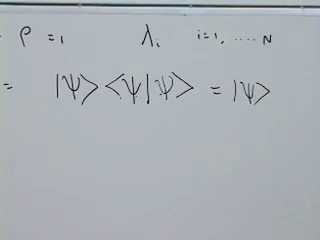
\includegraphics[width=0.72\textwidth]{lecture_08_figure_06.png}
\caption{純粋状態の密度行列は射影演算子として作用する：\(\rho\ket{\psi}=\ket{\psi}\)。}
\lectureframe{00:09:32}
\end{figure}

\section{トレースによる期待値}

密度行列に対する操作的な規則は
\begin{equation}
\overline{M}=\operatorname{Tr}(\rho M),
\end{equation}
である。ここで\(M\)は可観測量である。二つの因子については、トレースの巡回性により
\begin{equation}
\operatorname{Tr}(\rho M)=\operatorname{Tr}(M\rho),
\end{equation}
が成り立つ。\(\rho\)と\(M\)が可換であるかどうかによらない。

任意の正規直交基底\(\{\ket{i}\}\)において、
\begin{equation}
\operatorname{Tr}X=\sum_i\bra{i}X\ket{i}.
\end{equation}
数値は基底に依存しない。純粋状態に対しては、
\begin{align}
\overline{M}
&=\operatorname{Tr}\!\left(\ket{\psi}\bra{\psi}M\right) \\
&=\sum_i\braket{i}{\psi}\bra{\psi}M\ket{i} \\
&=\bra{\psi}M\left(\sum_i\ket{i}\bra{i}\right)\ket{\psi} \\
&=\bra{\psi}M\ket{\psi}.
\end{align}
恒等演算子の分解
\begin{equation}
\sum_i\ket{i}\bra{i}=I,
\end{equation}
により、密度行列の規則は見慣れた純粋状態の期待値に戻る。

\begin{figure}[htbp]
\centering
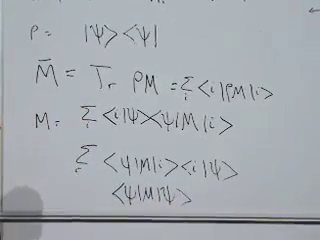
\includegraphics[width=0.74\textwidth]{lecture_08_figure_07.png}
\caption{純粋状態の射影演算子に対するトレース計算と恒等演算子の分解。}
\lectureframe{00:14:25}
\end{figure}

\begin{classroomqa}
\lecturetimestamp{00:14:38}
\audiencequestion{左辺の量は\(\overline{M}\)、すなわち\(M\)の平均であるべきか？}
\lecturerresponse{はい。トレースは演算子\(M\)そのものではなく、スカラーである期待値\(\overline{M}\)である。}
\end{classroomqa}

一般の密度行列に対しては、その固有基底を選ぶ：
\begin{equation}
\rho\ket{j}=\lambda_j\ket{j}.
\end{equation}
\(\rho\) と \(M\) の間に完全系を挿入する：
\begin{align}
\overline{M}
&=\sum_i\bra{i}\rho M\ket{i} \\
&=\sum_{i,j}\bra{i}\rho\ket{j}\bra{j}M\ket{i} \\
&=\sum_{i,j}\lambda_j\delta_{ij}\bra{j}M\ket{i} \\
&=\sum_j\lambda_j\bra{j}M\ket{j}.
\end{align}
これは通常の重み付き平均である：\(\lambda_j\) は \(j\) 番目の固有状態の確率であり、\(\bra{j}M\ket{j}\) はその状態における \(M\) の期待値である。

\begin{classroomqa}
\lecturetimestamp{00:18:12}
\audiencequestion{最後の行列要素でなぜ両方のラベルが \(j\) になるのか、そしてどの添字がまだ和を取られているのか。}
\lecturerresponse{この基底で \(\rho\) が対角であるため、\(\bra{i}\rho\ket{j}=\lambda_j\delta_{ij}\) となり、\(i=j\) の項だけが生き残る。元の二重和は一つの和に縮約され、それは \(j\) に関する和と呼んでよい。ダミーの和添字の名前には物理的意味はない。}
\end{classroomqa}

\section{欠落した情報としてのエントロピー}

古典確率分布 \(\{p_i\}\) に対して、次を定義する：
\begin{equation}
S=-\sum_i p_i\log p_i,
\end{equation}
ここで \(0\log 0\) はその極限値 \(0\) と解釈する。一つの確率が \(1\) に等しく、他がすべて消えるなら、\(S=0\) である：状態は既知である。\(n\) 個の可能性がすべて等確率なら、
\begin{equation}
p_i=\frac{1}{n},
\qquad
S=-n\left(\frac{1}{n}\log\frac{1}{n}\right)=\log n.
\end{equation}
したがってエントロピーは、確率分布がより多くの有意な可能性に広がるにつれて増大する。おおよそ、自然対数を用いる場合、\(e^S\) は同程度の重みをもつ状態の実効的な数である。

\begin{figure}[htbp]
\centering
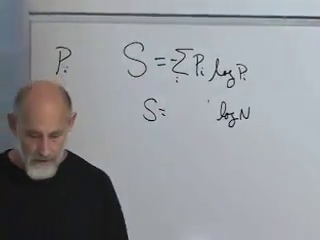
\includegraphics[width=0.68\textwidth]{lecture_08_figure_08.png}
\caption{確率分布に対するエントロピーと等確率の値 \(S=\log n\)。}
\lectureframe{00:21:08}
\end{figure}

密度行列に対しては、同じ定義をその固有値に適用する：
\begin{equation}
S(\rho)=-\sum_i\lambda_i\log\lambda_i
=-\operatorname{Tr}(\rho\log\rho).
\end{equation}
最初の表式は直ちに必要となるものであり、トレースの形は答えが基底に依存しないことを強調している。

\section{複合系と局所実験}

二つの部分系 \(A\) と \(B\) を考える。基底ベクトルを \(\ket{a,b}\) と書く。\(A\) が \(N\) 個の基底状態をもち、\(B\) が \(n\) 個をもつなら、複合系は \(Nn\) 個の基底状態をもつ。二つの系は同じである必要はない：一方が二状態のスピンで、他方が三状態の原子であってもよい。

この対の最も一般的な純粋状態は
\begin{equation}
\ket{\Psi}
=\sum_{a,b}\psi(a,b)\ket{a,b},
\qquad
\sum_{a,b}|\psi(a,b)|^2=1.
\end{equation}
である。ここでアリスが部分系 \(A\) にのみ作用する観測量 \(M_A\) を測定するとする。複合ヒルベルト空間上では演算子は \(M_A\otimes I_B\) である。その行列要素は
\begin{equation}
\bra{a',b'}M_A\otimes I_B\ket{a,b}
=\bra{a'}M_A\ket{a}\,\delta_{b'b}.
\end{equation}
である。\(B\) のラベルは受動的である。

期待値を完全に書くと：
\begin{align}
\expect{M_A}
&=\bra{\Psi}M_A\otimes I_B\ket{\Psi} \\
&=\sum_{a',b'}\sum_{a,b}
\psi^*(a',b')\psi(a,b)
\bra{a'}M_A\ket{a}\delta_{b'b} \\
&=\sum_{a',a,b}
\psi^*(a',b)\psi(a,b)
\bra{a'}M_A\ket{a}.
\end{align}

\begin{classroomqa}
\lecturetimestamp{00:29:12}
\audiencequestion{なぜブラのラベルにはプライムが付いているのに、ケットのラベルには付いていないのか。}
\lecturerresponse{行列要素を評価する前、ブラとケットは独立な和であるため、別々のダミーラベルを必要とする。プライムはブラの添字をケットの添字から区別する。その後、演算子と内積がそれらのラベルのどれが一致しなければならないかを決める。}
\end{classroomqa}

\(a\) と \(a'\) を固定して、\(b\) に関する和を実行する。結果は部分系 \(A\) 上の行列である：
\begin{equation}
\boxed{
\rho_A(a,a')
=\sum_b\psi(a,b)\psi^*(a',b)
}.
\end{equation}
これは \(A\) の縮約密度行列であり、等価に、純粋状態の射影演算子の \(B\) に関する部分トレースである：
\begin{equation}
\rho_A=\operatorname{Tr}_B\ket{\Psi}\bra{\Psi}.
\end{equation}
局所期待値は
\begin{equation}
\expect{M_A}
=\sum_{a,a'}\rho_A(a,a')\bra{a'}M_A\ket{a}
=\operatorname{Tr}_A(\rho_A M_A).
\end{equation}
となる。

\begin{figure}[htbp]
\centering
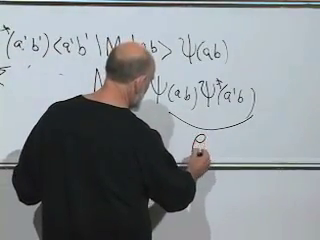
\includegraphics[width=0.76\textwidth]{lecture_08_figure_09.png}
\caption{\(B\) の添字は和を取られて消え、二つの \(A\) 添字をもつ行列が残る。}
\lectureframe{00:33:50}
\end{figure}

\begin{classroomqa}
\lecturetimestamp{00:35:39}
\audiencequestion{局所観測量は部分系 \(B\) 上の単なる恒等演算子なのか。}
\lecturerresponse{そのとおり。\(M_A\otimes I_B\) は \(A\) 座標を変えうるが、\(b\) を変えもせず、その他の形で依存もしない。だからその \(B\) 空間の行列要素は \(\delta_{b'b}\) なのである。}
\end{classroomqa}

したがって \(A\) に限定された実験に対するすべての予測は \(\rho_A\) に含まれる。ボブは自分の部分系を測定する必要はない。\(B\) の自由度を使わないというだけで、アリスの記述は密度行列の形に押し込まれる。

\section{純粋な全体は混合した部分をもちうる}

合成系は純粋状態 \(\ket{\Psi}\) にあるが、\(\rho_A\) は一般にいくつかの非零固有値をもつ。全体についての完全な知識は、各部分に対する状態ベクトルを意味しない。猫と銃は一つのもつれた状態ベクトルをもってよく、そのとき猫だけは縮約密度行列によって記述される。

\begin{classroomqa}
\lecturetimestamp{00:38:25}
\audiencequestion{\(\operatorname{Tr}(M\rho)\) を \((\operatorname{Tr}M)(\operatorname{Tr}\rho)\) で置き換えられるか。}
\lecturerresponse{いいえ。積のトレースは一般にトレースの積ではない。巡回性により \(\operatorname{Tr}(M\rho)=\operatorname{Tr}(\rho M)\) は許されるが、トレースが因数分解されるわけではない。}
\end{classroomqa}

\begin{classroomqa}
\lecturetimestamp{00:38:49}
\audiencequestion{我々は基底状態\(\ket{a,b}\)のみから始めたのか、それとも最も一般的な純粋状態から始めたのか。}
\lecturerresponse{複合系の最も一般的な純粋状態、すなわち\(\ket{\Psi}=\sum_{a,b}\psi(a,b)\ket{a,b}\)から始めた。単一の\(\ket{a,b}\)は一つの基底ベクトルにすぎない。驚くべきことは、この完全に指定された複合ベクトルでさえ混合還元状態を与えうることである。}
\end{classroomqa}

古典力学との対比は際立っている。複合系に関する完全な古典的情報は、その各座標を確定し、したがって各部分系を確定する。古典的確率分布は確かに周辺化されうるが、元の分布が一つの位相空間点に集中しているなら、すべての周辺分布もまた一つの確定した値に集中する。量子純粋状態は必ずしもその性質をもつ必要はない。

\begin{classroomqa}
\lecturetimestamp{00:40:46}
\audiencequestion{\(B\)について和をとることは、古典的な位置--速度分布を速度について積分することとどう異なるのか。}
\lecturerresponse{操作は似て見えるが、その純粋状態極限は異なる。完全に既知の古典的位相空間点は位置と速度の両方を確定するので、どちらの周辺分布も確定したままである。完全に既知のもつれ合った量子状態は、どちらの部分系についても非自明な混合状態を与えうる。したがって部分トレースは、純粋な全体から純粋な部分への古典的含意の量子的破綻を明らかにする。}
\end{classroomqa}

\section{積状態：例外的な場合}

\(\rho_A\)はいつ純粋なままでありうるか。答えは、波動関数が因数分解されなければならないということである：
\begin{equation}
\psi(a,b)=\phi(a)\chi(b).
\end{equation}
\(\phi\)と\(\chi\)はそれぞれ規格化されていると仮定する。還元密度行列に代入すると
\begin{align}
\rho_A(a,a')
&=\sum_b\phi(a)\chi(b)\phi^*(a')\chi^*(b) \\
&=\phi(a)\phi^*(a')\sum_b|\chi(b)|^2 \\
&=\phi(a)\phi^*(a').
\end{align}
したがって
\begin{equation}
\rho_A=\ket{\phi}\bra{\phi}.
\end{equation}
これは一つの固有値\(1\)をもち、残りの固有値はすべて\(0\)であり、エントロピーはゼロである。

\begin{figure}[htbp]
\centering
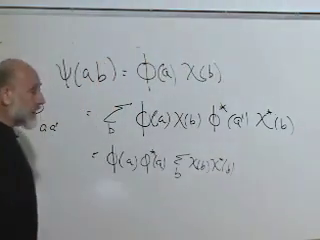
\includegraphics[width=0.74\textwidth]{lecture_08_figure_10.png}
\caption{因数分解された波動関数に対しては、\(B\)についての和は\(\chi\)の規格化に帰着する。}
\lectureframe{00:46:35}
\end{figure}

\begin{classroomqa}
\lecturetimestamp{00:44:17}
\audiencequestion{\(\phi(a)\)自体が\(A\)系の状態なのか。}
\lecturerresponse{それはその状態の波動関数成分である。より明示的には、\(\ket{\phi}=\sum_a\phi(a)\ket{a}\)であり、同様に\(\ket{\chi}=\sum_b\chi(b)\ket{b}\)である。因数分解とは\(\ket{\Psi}=\ket{\phi}\otimes\ket{\chi}\)、すなわち\(A\)と\(B\)の間にもつれ合いのない積状態を意味する。}
\end{classroomqa}

すべての局所可観測量に対して、
\begin{equation}
\expect{M_A}
=\operatorname{Tr}(\rho_A M_A)
=\bra{\phi}M_A\ket{\phi}.
\end{equation}
部分系\(A\)は純粋状態\(\ket{\phi}\)と全く同じように振る舞う。二部分純粋状態に対して、\(\rho_A\)のエントロピーはしたがって積構造を検査する：ゼロは積状態を意味し、非ゼロのエントロピーはもつれ合いを意味する。ゼロに近い値は弱いもつれ合いを示し、最大値に近い値はこの二分割を横断するいかなる積からも遠い状態を示す。

\section{一重項：純粋な全体と最大の局所無知}

二スピン一重項
\begin{equation}
\ket{\Psi^-}
=\frac{1}{\sqrt{2}}
\left(
\ket{\uparrow\downarrow}
-\ket{\downarrow\uparrow}
\right).
\end{equation}
をとる。その非ゼロの波動関数成分は
\begin{equation}
\psi(\uparrow,\downarrow)=\frac{1}{\sqrt{2}},
\qquad
\psi(\downarrow,\uparrow)=-\frac{1}{\sqrt{2}},
\end{equation}
であり、一方\(\psi(\uparrow,\uparrow)=\psi(\downarrow,\downarrow)=0\)である。

スピン\(2\)についてトレースをとる。対角成分は
\begin{align}
\rho_1(\uparrow,\uparrow)
&=|\psi(\uparrow,\uparrow)|^2
 +|\psi(\uparrow,\downarrow)|^2
=\frac{1}{2}, \\
\rho_1(\downarrow,\downarrow)
&=|\psi(\downarrow,\uparrow)|^2
 +|\psi(\downarrow,\downarrow)|^2
=\frac{1}{2}.
\end{align}
非対角成分は
\begin{align}
\rho_1(\uparrow,\downarrow)
&=\psi(\uparrow,\uparrow)\psi^*(\downarrow,\uparrow)
 +\psi(\uparrow,\downarrow)\psi^*(\downarrow,\downarrow) \\
&=0,
\end{align}
であり、その複素共役もまた消える。したがって
\begin{equation}
\rho_1
=
\begin{pmatrix}
\frac12&0\\[2pt]
0&\frac12
\end{pmatrix}
=\frac12 I.
\end{equation}

\begin{figure}[htbp]
\centering
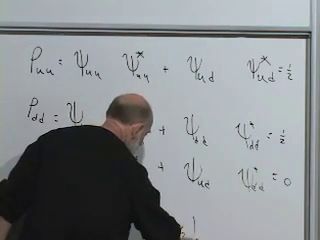
\includegraphics[width=0.76\textwidth]{lecture_08_figure_11.png}
\caption{一重項における一つのスピンの還元密度行列の四つの成分。}
\lectureframe{00:55:35}
\end{figure}

\begin{classroomqa}
\lecturetimestamp{00:55:58}
\audiencequestion{単一スピン還元状態のエントロピーは何か。}
\lecturerresponse{その二つの固有値はともに\(1/2\)であるので、
\[
S_1=-2\left(\frac12\log\frac12\right)=\log 2.
\]
これは二状態部分系に利用可能な最大エントロピーである。最大混合状態を特徴づけるのは、任意の基底における等しい行列成分ではなく、等しい\emph{固有値}である。}
\end{classroomqa}

スピン期待値はあらゆる軸に沿って消える：
\begin{equation}
\expect{\bm{\sigma}\cdot\hat{\bm n}}
=\operatorname{Tr}\!\left(
\rho_1\,\bm{\sigma}\cdot\hat{\bm n}
\right)
=\frac12\operatorname{Tr}
\left(\bm{\sigma}\cdot\hat{\bm n}\right)
=0.
\end{equation}

\begin{classroomqa}
\lecturetimestamp{00:58:37}
\audiencequestion{なぜ\(\bm{\sigma}\cdot\hat{\bm n}\)のトレースはあらゆる方向に対してゼロなのか。}
\lecturerresponse{各パウリ行列はトレースがゼロである。\(\bm{\sigma}\cdot\hat{\bm n}=n_1\sigma_1+n_2\sigma_2+n_3\sigma_3\)であるので、トレースの線形性により任意の単位ベクトル\(\hat{\bm n}\)に対してゼロとなる。したがってスピンは、選ばれた任意の軸に対して平行または反平行に見出される確率が等しい。}
\end{classroomqa}

対全体は確定した純粋状態をもち、エントロピーはゼロである。どちらのスピンも単独では最大混合である。これは欠陥のある準備記録によって引き起こされた無知ではなく、もつれ合いによって含意される局所状態である。

\section{等振幅積状態}

次に
\begin{equation}
\ket{\Phi}
=\frac12\left(
\ket{\uparrow\uparrow}
+\ket{\uparrow\downarrow}
+\ket{\downarrow\uparrow}
+\ket{\downarrow\downarrow}
\right).
\end{equation}
を考える。四つの振幅はすべて\(1/2\)に等しいので、規格化は\(1/4\)の四つの寄与から従う。スピン\(2\)についてトレースをとると
\begin{equation}
\rho_1
=
\begin{pmatrix}
\frac12&\frac12\\[2pt]
\frac12&\frac12
\end{pmatrix}.
\end{equation}
が得られる。そのトレースは\(1\)であるが、
\begin{equation}
\det\rho_1
=\frac14-\frac14
=0.
\end{equation}

\begin{classroomqa}
\lecturetimestamp{01:02:23}
\audiencequestion{ここで、トレースと行列式はどのようにして2つの固有値を決定するのですか。}
\lecturerresponse{\(2\times2\)行列では、固有値の和がトレースであり、その積が行列式である。したがって\(\lambda_1+\lambda_2=1\)および\(\lambda_1\lambda_2=0\)となり、組\(\{1,0\}\)が強制される。縮約状態は純粋であり、そのエントロピーはゼロである。}
\end{classroomqa}

\begin{classroomqa}
\lecturetimestamp{01:03:18}
\audiencequestion{もつれていない2つのスピンは実際には何をしているのですか。}
\lecturerresponse{それらはどちらも正の\(x\)軸に沿って整列している。この答えは因数分解によって認識できる。
\[
\ket{\Phi}
=\frac{\ket{\uparrow}+\ket{\downarrow}}{\sqrt2}
\otimes
\frac{\ket{\uparrow}+\ket{\downarrow}}{\sqrt2},
\]
または、パウリ期待値を計算することによって実験的に確立できる。}
\end{classroomqa}

\(z\)成分については、
\begin{equation}
\sigma_3=
\begin{pmatrix}
1&0\\[2pt]
0&-1
\end{pmatrix},
\qquad
\operatorname{Tr}(\rho_1\sigma_3)=0.
\end{equation}
\(x\)成分については、
\begin{equation}
\sigma_1=
\begin{pmatrix}
0&1\\[2pt]
1&0
\end{pmatrix},
\end{equation}
および
\begin{align}
\rho_1\sigma_1
&=
\begin{pmatrix}
\frac12&\frac12\\[2pt]
\frac12&\frac12
\end{pmatrix}
\begin{pmatrix}
0&1\\[2pt]
1&0
\end{pmatrix}
=
\begin{pmatrix}
\frac12&\frac12\\[2pt]
\frac12&\frac12
\end{pmatrix}, \\
\operatorname{Tr}(\rho_1\sigma_1)&=1.
\end{align}

\begin{figure}[htbp]
\centering
\includegraphics[width=0.70\textwidth]{lecture_08_figure_03.png}
\caption{等振幅の縮約状態に対する\(\sigma_1\)行列の計算。}
\lectureframe{01:05:13}
\end{figure}

したがって\(\expect{\sigma_1}=1\)である一方、\(\expect{\sigma_2}=\expect{\sigma_3}=0\)である。振幅を厳密な因数分解からずらすと、一般に固有値は\(\{1,0\}\)から2つの非ゼロ値へと変化する。その結果生じる小さなエントロピーは、少量のもつれを測っている。

\section{それは誰のエントロピーか}

いま計算したエントロピーは部分系に属する。一重項の例では、
\begin{equation}
S(\rho_{12})=0,
\qquad
S(\rho_1)=S(\rho_2)=\log 2.
\end{equation}
全体は純粋である一方、各部分は混合である。したがって、もつれエントロピーは素朴な加法則\(S_{12}=S_1+S_2\)に従わない。二部分純粋状態では、2つの縮約密度行列は同じ非ゼロ固有値をもつので、全体のエントロピーが消えるにもかかわらず、それらのエントロピーは等しい。

\begin{classroomqa}
\lecturetimestamp{01:09:03}
\audiencequestion{すべての密度行列は最終的にもつれ密度行列なのですか。}
\lecturerresponse{操作上は、欠落した記録を何が担っているかを追跡することなく、通常の不確定性を記述してよい。準備装置、環境、または観測者を含めれば、その不確定性はしばしば、観測されない自由度とのもつれとして見なせる。数学的にはこの考えは厳密である。すべての密度行列はより大きなヒルベルト空間上の純化を許すが、その純化は物理的な準備履歴を一意に特定するものではない。}
\end{classroomqa}

\section{離散的な古典的運動から量子運動へ}

ここで一時的にもつれを離れ、状態が時間とともにどのように変化するかを問う。有限個の配置をもつ古典系では、可逆な発展は置換である。各状態には1つの後続状態と1つの先行状態があり、運動はサイクルに分解される。

\begin{figure}[htbp]
\centering
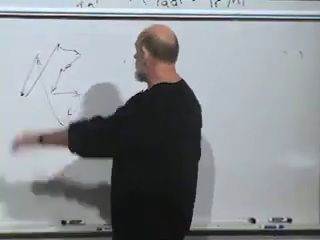
\includegraphics[width=0.70\textwidth]{lecture_08_figure_12.png}
\caption{離散的な配置間の矢印で表された古典的可逆発展。}
\lectureframe{01:11:40}
\end{figure}

\begin{classroomqa}
\lecturetimestamp{01:11:51}
\audiencequestion{配置が離散的なら、なぜ時間ステップも離散的でなければならないのですか。}
\lecturerresponse{厳密に古典的な2状態模型には、連続的な経路が通過しうる中間配置が存在しない。物理的なコインをゆっくり回すと、その向きが追加の連続座標として導入されるので、もはや2配置模型ではない。量子的な2状態系は異なる。そのヒルベルト空間は、正規直交基底が2つの要素しかもたなくても、連続的な重ね合わせの族を含む。}
\end{classroomqa}

スピン\(\tfrac12\)状態は、重ね合わせを通じて\(\ket{\uparrow}\)から\(\ket{\downarrow}\)へ連続的に回転できる。有限次元は、状態ベクトルの有限集合を意味しない。これにより、離散的な量子系で連続的な時間発展が可能になる。

可逆な微視的力学は区別も保存する。2つの異なる古典的初期条件が1つの微視的状態に合流することはない。それはどの初期条件が生じたかを消去してしまうからである。ハミルトン力学では、この可逆性にはリウヴィルの定理が伴う。すなわち、位相空間の体積は保存される。

\begin{classroomqa}
\lecturetimestamp{01:15:26}
\audiencequestion{複数の初期条件が同じ定常状態に近づく非線形分岐についてはどうですか。}
\lecturerresponse{アトラクターは、環境の自由度が捨て去られた有効散逸的記述に現れる。基礎的な微視的ハミルトン発展は可逆のままであり、情報は観測されない変数へ移されうるが、異なる完全状態が文字通り1つの完全状態になるわけではない。}
\end{classroomqa}

量子的な言明はユニタリ性である。直交する初期状態は直交する最終状態へ発展し、より一般にはすべての内積が保存される。

\begin{classroomqa}
\lecturetimestamp{01:16:50}
\audiencequestion{二つの状態はまったく同じ影響を受けなければならないのか。\(z\)上向きと\(z\)下向きの初期状態は、\(x\)方向の磁場中でどうなるのか。}
\lecturerresponse{同じ時間発展演算子が両方の状態に作用しなければならない。横磁場中で二つのスピンは歳差運動するが、それらのブロッホベクトルは逆向きのままであり、状態ベクトルは直交したままである。異なる外部履歴を適用することは、異なる時間発展演算子を比較することにほかならない。}
\end{classroomqa}

\section{線形性とユニタリ性}

量子の時間発展の第一原理は線形性である。
\begin{equation}
\ket{\psi(t)}=U(t)\ket{\psi(0)}.
\end{equation}
演算子は経過時間に依存し、次を満たす。
\begin{equation}
U(0)=I.
\end{equation}
量子力学そのものの線形性と同様に、この規則はその経験的成功によって正当化される。

\begin{figure}[htbp]
\centering
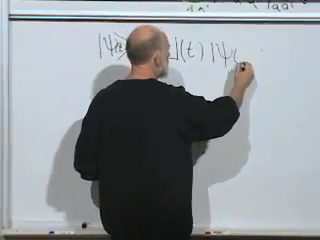
\includegraphics[width=0.70\textwidth]{lecture_08_figure_13.png}
\caption{時刻\(t\)における状態は、初期状態に作用する線形演算子\(U(t)\)によって得られる。}
\lectureframe{01:19:00}
\end{figure}

\begin{classroomqa}
\lecturetimestamp{01:19:01}
\audiencequestion{\(U(t)\)は\(t=0\)において何でなければならないか。}
\lecturerresponse{恒等演算子でなければならない。経過時間がゼロのとき、あらゆる可能な初期ベクトルに対して状態は変化しない。}
\end{classroomqa}

第二の原理は内積の保存である。
\begin{equation}
\braket{\phi(t)}{\psi(t)}
=\braket{\phi(0)}{\psi(0)}.
\end{equation}
\(\phi=\psi\)のとき、これは規格化を、したがって全確率を保存する。初期状態が直交しているとき、これは完全な識別可能性を保存する。任意の状態に対しては、それらの幾何学的関係の全体を保存する。

ブラは次に従って発展する。
\begin{equation}
\bra{\phi(t)}
=\bra{\phi(0)}U^\dagger(t),
\end{equation}
したがって
\begin{align}
\braket{\phi(t)}{\psi(t)}
&=\bra{\phi(0)}U^\dagger(t)U(t)\ket{\psi(0)} \\
&=\braket{\phi(0)}{\psi(0)}.
\end{align}
この等式があらゆる初期ベクトルの組に対して成り立つので、
\begin{equation}
\boxed{U^\dagger(t)U(t)=I}.
\end{equation}

\begin{figure}[htbp]
\centering
\includegraphics[width=0.74\textwidth]{lecture_08_figure_04.png}
\caption{ケットの発展、ブラの発展、そして\(U^\dagger U=I\)を導く内積条件。}
\lectureframe{01:23:30}
\end{figure}

\begin{classroomqa}
\lecturetimestamp{01:22:10}
\audiencequestion{なぜブラは\(U\)ではなく\(U^\dagger\)を獲得するのか。}
\lecturerresponse{エルミート共役をとると因子の順序が逆になり、各演算子がそのエルミート共役に置き換わる。
\[
\bigl(U\ket{\phi}\bigr)^\dagger
=\bra{\phi}U^\dagger.
\]
これが、整合的な内積に必要な双対的な作用である。}
\end{classroomqa}

\begin{classroomqa}
\lecturetimestamp{01:24:34}
\audiencequestion{もし\(U\)が単なる複素数であったなら、\(U^\dagger U=1\)は何を意味するのか。}
\lecturerresponse{それは\(|U|=1\)を意味するので、\(U=e^{i\theta}\)は単位円上にある。ユニタリ行列は純粋な位相の演算子版であり、長さと内積を保存する。}
\end{classroomqa}

\section{微小発展とハミルトニアン}

\(\epsilon\)を非常に短い時間間隔とする。\(U(0)=I\)であるから、一次の展開を
\begin{equation}
U(\epsilon)=I-i\epsilon h+O(\epsilon^2).
\end{equation}
と書く。負号と\(i\)の因子は便利な慣習である。エルミート共役をとると
\begin{equation}
U^\dagger(\epsilon)
=I+i\epsilon h^\dagger+O(\epsilon^2).
\end{equation}
が得られる。するとユニタリ性は
\begin{align}
I
&=U^\dagger(\epsilon)U(\epsilon) \\
&=\left(I+i\epsilon h^\dagger\right)
\left(I-i\epsilon h\right)+O(\epsilon^2) \\
&=I+i\epsilon(h^\dagger-h)+O(\epsilon^2).
\end{align}
を要求する。一次の項は消えなければならない。
\begin{equation}
\boxed{h^\dagger=h}.
\end{equation}
微小生成子はエルミートである。

\begin{figure}[htbp]
\centering
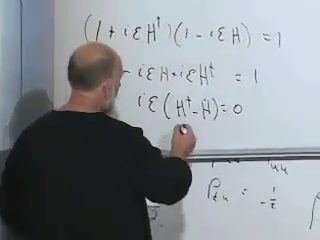
\includegraphics[width=0.76\textwidth]{lecture_08_figure_14.png}
\caption{一次のユニタリ性は、微小生成子がエルミートであることを強制する。}
\lectureframe{01:29:35}
\end{figure}

上記の暫定的な慣習では、\(h\)は角振動数の単位をもつ。物理的単位を復元し、エネルギー演算子を
\begin{equation}
H=\hbar h.
\end{equation}
と定義する。このエルミート演算子がハミルトニアンであり、その固有値がエネルギー準位である。

微小演算子を状態に作用させる。
\begin{equation}
\ket{\psi(\epsilon)}
=\left(I-\frac{i\epsilon}{\hbar}H\right)\ket{\psi(0)}
+O(\epsilon^2).
\end{equation}
初期状態を引き、\(\epsilon\)で割り、極限をとる。
\begin{equation}
\frac{\mathrm d}{\mathrm dt}\ket{\psi(t)}
=-\frac{i}{\hbar}H\ket{\psi(t)}.
\end{equation}
等価的に、
\begin{equation}
\boxed{
i\hbar\frac{\mathrm d}{\mathrm dt}\ket{\psi(t)}
=H\ket{\psi(t)}
}.
\end{equation}
これが一般のSchr\"odinger方程式である。

\begin{figure}[htbp]
\centering
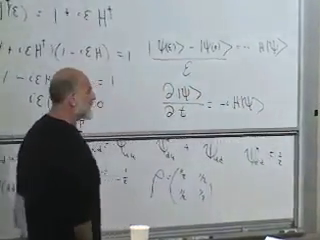
\includegraphics[width=0.76\textwidth]{lecture_08_figure_15.png}
\caption{微小な差分商が状態の時間微分になる。}
\lectureframe{01:32:18}
\end{figure}

ハミルトニアンは物理的設定に依存する。外部磁場や他の制御が変化すれば、時間とともに変化しうる。設定が時間に依存しないとき、\(H\)は固定されたエルミート演算子である。

\begin{classroomqa}
\lecturetimestamp{01:34:30}
\audiencequestion{内積の保存は、初期にもつれていない系がもつれないままでなければならないことを意味するのか。}
\lecturerresponse{いいえ。ユニタリ性が保存するのは完全な状態ベクトル間の内積であり、選ばれた分割の積構造ではない。相互作用ハミルトニアンは積状態を絡み合った状態へと移しうる。もしユニタリ演算子がこれをなしえないなら、測定は系を装置と相関させることができないであろう。}
\end{classroomqa}

\section{エントロピーの単位}

\begin{classroomqa}
\lecturetimestamp{01:35:08}
\audiencequestion{もつれはジュールのような物理的単位をもつのか。}
\lecturerresponse{もつれエントロピーは情報の尺度であり、エネルギーではない。自然対数を用いればナットで測られ、二を底とする対数を用いればビットで測られる。どちらも無次元の計数の慣習である。}
\end{classroomqa}

熱力学の記法はこの点を曖昧にしうる。なぜならボルツマン定数は、ケルビンで測った温度とエネルギーとの間を変換するからである：
\begin{equation}
\expect{K}_{\mathrm{monatomic}}
=\frac32 k_{\mathrm B}T.
\end{equation}
可逆熱の関係は
\begin{equation}
\delta Q_{\mathrm{rev}}=T\,\mathrm dS_{\mathrm{th}}.
\end{equation}
情報エントロピーが
\begin{equation}
S_{\mathrm{info}}=-\sum_i p_i\log p_i,
\end{equation}
であるなら、従来の熱力学的エントロピーは
\begin{equation}
S_{\mathrm{th}}=k_{\mathrm B}S_{\mathrm{info}}.
\end{equation}
である。\(k_{\mathrm B}=1\)と置くと温度をエネルギーの単位で測ることになり、エントロピーは無次元のままである。そのときボルツマン定数は、新たな種類のもつれの単位ではなく、変換因子として認識される。ボルツマンの統計的考えをブラウン運動に関するアインシュタインの1905年の仕事と結びつける歴史的な余談は、情報理論的な定義を変えるものではない。

\section{エネルギー固有状態と位相}

\begin{classroomqa}
\lecturetimestamp{01:39:54}
\audiencequestion{なぜエルミート生成子\(H\)がエネルギーと同一視されるのか。}
\lecturerresponse{ユニタリ性だけから証明されるのは、生成子がエルミートであることだけである。それをエネルギーと同一視することは追加の物理的命題である。すなわち、エネルギーが時間並進を生成する。時間に依存しないハミルトニアンに対しては、発展を支配する同じ演算子が保存され、その固有値が定常エネルギー準位である。具体的なハミルトニアンが、その同一視の実験的内容を与える。}
\end{classroomqa}

プランク定数と振動数の関係は
\begin{equation}
E=h\nu=\hbar\omega,
\qquad
\omega=2\pi\nu,
\qquad
h=2\pi\hbar.
\end{equation}

\begin{classroomqa}
\lecturetimestamp{01:40:30}
\audiencequestion{発展方程式には\(h\)、\(\hbar\)、それとも余分な因子\(2\pi\)が含まれるべきか。}
\lecturerresponse{角振動数\(\omega\)を用いると、方程式は\(E=\hbar\omega\)であり、Schr\"odinger方程式には\(\hbar\)が含まれる。通常の振動数\(\nu\)を用いると、等価な関係は\(E=h\nu\)である。因子\(2\pi\)は\(\omega=2\pi\nu\)と\(h=2\pi\hbar\)によって完全に説明される。}
\end{classroomqa}

初期状態がエネルギー固有ベクトルであるとしよう：
\begin{equation}
H\ket{\psi(0)}=E\ket{\psi(0)}.
\end{equation}

\begin{classroomqa}
\lecturetimestamp{01:43:18}
\audiencequestion{状態がエネルギー固有ベクトルのままであれば、それは変化しないという意味か。}
\lecturerresponse{時間に依存する複素因子を獲得し、同じ固有値をもつ固有ベクトルのままでありうる。ユニタリ性はその因子を位相に制限する。したがって、ケットが位相の中で回転している間も、レイは定常である。}
\end{classroomqa}

次のように書く：
\begin{equation}
\ket{\psi(t)}=f(t)\ket{\psi(0)}.
\end{equation}

\begin{figure}[H]
\centering
\includegraphics[width=0.70\textwidth]{lecture_08_figure_05.png}
\caption{エネルギー固有状態は、スカラー因子\(f(t)\)を除いて同じヒルベルト空間の方向にとどまる。}
\lectureframe{01:43:54}
\end{figure}

Schr\"odinger方程式に代入すると
\begin{align}
i\hbar\frac{\mathrm d f}{\mathrm dt}\ket{\psi(0)}
&=f(t)H\ket{\psi(0)} \\
&=E f(t)\ket{\psi(0)}.
\end{align}
共通のベクトルを消去する：
\begin{equation}
\frac{\mathrm d f}{\mathrm dt}
=-\frac{iE}{\hbar}f(t).
\end{equation}
\(f(0)=1\)として、
\begin{equation}
f(t)=e^{-iEt/\hbar},
\qquad
\ket{\psi(t)}=e^{-iEt/\hbar}\ket{\psi(0)}.
\end{equation}

\begin{figure}[H]
\centering
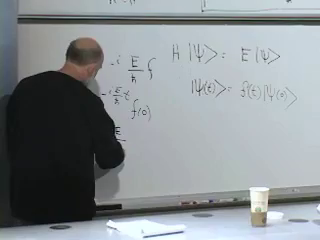
\includegraphics[width=0.76\textwidth]{lecture_08_figure_16.png}
\caption{エネルギー固有値方程式と、それから生じる位相の発展。}
\lectureframe{01:46:10}
\end{figure}

\begin{classroomqa}
\lecturetimestamp{01:45:39}
\audiencequestion{位相\(e^{-iEt/\hbar}\)における\(t\)の係数は何か。}
\lecturerresponse{それは角振動数であり、
\[
\omega=\frac{E}{\hbar}.
\]
等価に\(E=\hbar\omega\)である。実の指数係数ならば成長率または減衰率を表すであろうが、ここでの虚の指数はユニタリな位相回転を表す。}
\end{classroomqa}

この位相と振動数の関係とSchr\"odinger方程式は、同じ時間発展の法則の二つの形である。方程式は一般的であり、自由粒子、ポテンシャル中の粒子、磁場中のスピンは、それぞれのハミルトニアンによって異なる。それらのハミルトニアンを選び、解くことが次の段階である。
